\documentclass[a4paper,english,titlepage]{article}

\usepackage{mathcomp,amssymb,mathptm,verimagstudent}
\usepackage[utf8]{inputenc}
\usepackage[T1]{fontenc}
\usepackage{algorithm}
\usepackage{algorithmic}
\newtheorem{definition}{Definition}[section]
\newtheorem{theorem}{Theroem}[section]
\usepackage{stmaryrd}
\usepackage{graphicx}

\title{Temporal Data Mining : Learning From Positive Examples}
\author{Ahmed-Antoine \textsc{Bouhemad}}
\date{4 juillet 2019}
\shorttitle{Data Clustering}
\institute{\textsc{VERIMAG}}
\abstract{
During my internship I worked on Data Clustering. This task aims to analyse data, by dividing it in set of differents structures, using common features which correspond to a spatial similarity. This technique is used in many fields including image analysis, bioinformatics, machine learning. }
\keywords{Data Clustering, Data mining}
\tutor{Thao \textsc{Dang} \\ Nicolas \textsc{Basset}}
\webaddress{https://github.com/ahmedAnB/Data-clustering}
\reporttype{Internship}

\begin{document}
  	
  \maketitlepage
  	

  
  \tableofcontents
  
  	\clearpage
 	\newpage
 	\mbox{~}
 	\clearpage
 	\newpage

	\part{Contexte}

	Dans cette partie nous allons montrer quels ont été les principes pour générer N points en D dimenions. Pour vérifier la cohérence des algorithmes, les points ont été générés à partir de differents clusters initiaux.
	Ces clusters initiaux peuvent être de differentes formes : des rectangles de tailles differentes ou des cercles de rayons differents \\
	Le code utilisé pour cette partie est dans le fichier \textsc{creation\_point.py}
	
	\section{Génération de Rectangles}
	Les fonctions utlisées pour générer les rectangles sont :  \textsc{creation\_point\_rectangles(nb\_point, nb\_rectangle, dimension)} et \textsc{creation\_point\_rectangles\_2(nb\_point, nb\_rectangle, dimension)}.\\
	Ci-après, le pseudo-code correspondant.

	\begin{algorithm}
		\caption{Générer N points dans $n_{rectangles}$ en D dimensions}
	\begin{algorithmic}
		\REQUIRE $N \geq 0 $, $n_{rect} \geq 0 $, $D \geq 0$
		\ENSURE liste de N points répartis dans $n_{rect}$ rectangles
		\STATE $m \leftarrow \lfloor\frac{N}{n_{rect}}\rfloor$
		\STATE $points \leftarrow [\ ]$
		\FOR{$j\in \llbracket 1, n_{rect}\rrbracket $}
		\STATE $cote \leftarrow$ génération d'une liste de D nombre aléatoie dans ]0, 0.5]
		\STATE sauvergarde des sommets et des cotés qui permettent de representer des carrés
		\FOR {$i \in \llbracket 1, m\rrbracket$}
		\STATE $point \leftarrow $ génére un point dans le rectangle j
		\STATE on stocke le points dans la listes points
		\ENDFOR
		\ENDFOR
		\STATE \textbf{return} points, carrés
	\end{algorithmic}
\end{algorithm}
	\begin{center}
	\begin{figure}[h!]
		\includegraphics[scale=0.35]{exemple_rectangles.png}
		\includegraphics[scale=0.35]{exemples_cercles.png}
		\caption{Génération de points sur 10 rectangles et de cercles}
  \end{figure}
  \end{center}  
  \section{Génération de cercles}
  Les fonctions utilisées pour générer les cercles ressemblent fortement à celle pour les rectangles qui sont : \textsc{creation\_point\_cercles} et \textsc{creation\_point\_sur\_cercle}. Cette dernière fonction permettant de générer des points de manière uniforme sur un cercle. 
	  Nous allons décrire l'algorithme utilisé pour cette génération uniforme.\\

	\begin{algorithm}
		\caption{Générer N points dans $n_{cerlces}$ en D dimensions}
	\begin{algorithmic}
		\REQUIRE $N \geq 0 $, $n_{cercles} \geq 0 $, $D \geq 0$
		\ENSURE liste de N points répartis dans $n_{rect}$ cercles
		\STATE $m \leftarrow \lfloor\frac{N}{n_{rect}}\rfloor$
		\STATE $points \leftarrow [\ ]$
		\FOR{$j\in \llbracket 1, n_{cerlces}\rrbracket $}
		\STATE $rayon \leftarrow$ uniform(0.1, 0.3)
		\STATE $center \leftarrow$ point aléatoire en D dimensions
		\FOR {$i \in \llbracket1, m\rrbracket$}
		\STATE $point \leftarrow $ génére un point dans le cercle j
		\STATE $point_{cercle} =$ [center[i] +$(xi - center[i])\times \frac{rayon}{distance(point,\ center)}$  for i, xi in enumerate($point$)]
		\ENDFOR
		\ENDFOR
		\STATE \textbf{return} points, carrés
	\end{algorithmic}
\end{algorithm}

\begin{figure}[h!]
		\hspace*{0mm}\vfill
		\begin{center}	
		\includegraphics[scale=0.35]{exemple_sur_cercle.png}
		\caption{Génération de points sur deux cercles}
 		\end{center}  
		\vfill\hspace*{0mm}	
	\end{figure}
\newpage
	\part{Résolution du problème}
Dans cette partie, nous allons voir la mise en place pour régler le problème de partionnement de données. 
C'est-à-dire comment l'algoritme a réussi à comprendre quelles sont les points qui étaient assez proches pour former un cluster. 
Dans notre algorithme les clusters seront des rectangles et l'algorithme devra rendre les clusters optimaux qu'il a trouvé. 
Il faut que le nombre de clusters soit minimal et qu'ils occupent le moins d'espace possible.\\
Pour résoudre ce problème, l'algorithme développé va dans un premier temps créer une table hachage qui permettra de partitionner l'espace en un quadrillage,
puis l'algorithme en déduira un premier ensemble de rectangles, 
enfin l'algoritme appliquera une méthode des plus proches voisins afin d'avoir le nombre optimal de clusters.
Le code se trouve dans le fichier \textsc{main.py} pour la première version de l'algorithme des plus proches voisins et la création de la table de hachage.
	\section{Création de la table de hachage}
L'algorithme générant la table de hachage fonctionne ainsi : pour chaque point, il va créer une clef qui va dépendre des coordonnées du point, et si les points ont la même clef,

on pourra en déduire qu'ils sont proches les uns des autres et ils vont donc appartenir au même ensemble de points stockés dans la table de hachage pour la clef correspondante.\\

Cette algorithme est de complexité $O(N\times D)$
		\begin{algorithm}
		\caption{Créer une table de hachage regroupant des points proches}
	\begin{algorithmic}
		\REQUIRE $points \neq \emptyset$,  $D \geq 0$, $ \epsilon > 0$
		\ENSURE table de hachage
		\STATE $m \leftarrow \lfloor\frac{N}{n_{rect}}\rfloor$
		\STATE $HT \leftarrow \{\ \} $,
		\FOR{$point = ( x_1, ... ,x_D ) \in points$}
		\STATE $lower = (\lfloor \frac{x_i}{\epsilon} \rfloor)_{ \forall i \in \llbracket 1,D \rrbracket}$
		\IF {$lower \in HT.keys$}
		\STATE On ajoute point à $HT[lower]$
		\ELSE 
		\STATE $HT[lower] = [point]$
		\ENDIF
		\ENDFOR
		\STATE \textbf{return} HT
	\end{algorithmic}
	\end{algorithm}


 	\section{Déduction des rectangles minimums}
Pour trouver un premier ensemble de clusters, on va extraire chaque clef de la table de hachage afin d'en déduire une bounding box pour les points appartenants à une même clef.
Afin d'avoir cette bounding il suffit de prendre le rectangle le plus petit qui contient tout les points en question.

	\section{Algorithme des plus proches voisins}
	On applique ensuite l'algoritme des plus proches voisins qui va nous retrouver les deux rectangles les plus proches. 
	Cet algorithme est un algorithme naïf car il va tester tous les voisins possibles afin de déduire le plus proche. 
	Il est en complexité $O(n_{cluster}^{2})$ mais nous l'avons choisit, car en dimensions importantes il est plus efficaces que d'algorithmes tels que k-means, kd-tree.
		\begin{algorithm}
		\caption{Retourner les rectangles les plus proches}
		\begin{algorithmic}
			\REQUIRE $set_{rectangles} \neq \emptyset$,  $D \geq 0$
		\ENSURE couple de rectangles les plus proches
		\STATE $nearest \leftarrow \{set_{rectangles}[0], set_{rectangles}[1]\}$
		\STATE $min\_distance \leftarrow distance(set_{rectangles}[0], set_{rectangles}[1])$,
		\FOR{$i  \in \llbracket 0, n-1 \rrbracket $}
		\FOR{$j \in \llbracket i +1, n-1\rrbracket$}
		\STATE $dist = distance(set_{rectangles}[i], set_{rectangles}[j])$
		\IF {$dist < min\_dist$}
		\STATE $nearest \leftarrow \{set_{rectangles}[i], set_{rectangles}[j]\}$
		\STATE $min\_distance \leftarrow dist$
		\ENDIF
		\ENDFOR
		\ENDFOR
		\STATE \textbf{return} nearest
	\end{algorithmic}
	\end{algorithm}


	\section{Conditions d'arrêt}
Pour l'instant, la condition d'arrêt mise en place repose sur le nombre de clusters que l'utilisateur veut en sortie. 
Cependant, on pourra utiliser une condition d'arrêt portant sur l'évolution d'une fonction de coût en fonction du nombre de cluster et choisir le nombre de cluster minimisant la fonction et n'étant pas trop grand. 
  
	\section{Exemple d'évolution de l'algorithme}  
Afin de visualiser l'algorithme j'ai mis en place une bibliothèque permettant d'afficher les points et les rectangles dans \textsc{affichage\_point.py}.
  	
\begin{figure}[h!]
		\includegraphics[scale=0.35]{1_1.png}
		\includegraphics[scale=0.35]{89.png}
		\includegraphics[scale=0.35]{101.png}
		\caption{Visualisation de l'algorithme pour un ensemble de clusters initiaux carrés}
 	\end{figure}
  	\begin{figure}[h!]
		\includegraphics[scale=0.35]{1.png}
		\includegraphics[scale=0.35]{77.png}
		\includegraphics[scale=0.35]{109.png}
		\includegraphics[scale=0.35]{126.png}	
	\caption{Visualisation de l'algorithme pour un ensemble de clusters initiaux en forme de rectangles}
	\label{evo_algo}
	\end{figure}

 
	\section{Optimisation Nearest Neighboor}
Pour optimiser le temps de l'algorithme du plus proche voisins, on a mit en place un système de liste trièe 
ayant une initialisation en complexité quadratique mais pour 
la mise à jour et trouver le minimum la complexité est en $O(n\log{n}) $.
	\clearpage
 	\newpage

\part{Résultats}

\section{Réalisation des expériences}
Pour tester les algorithmes et donc évaluer les performances en fonction de différentes caractéristiques, on a réalisé des expériences dont on peut voir les résultats ci-après.
Les fonctions pour tester les algorithmes ce trouvent dans \textsc{tests.py} et \textsc{experiences.py}.

\subsection{$1^{ère}$ expérience}
On a évalué le taux d'erreur, pour différentes initialisations de l'algorithme et differents nombres de clusters initiaux.\\
\subsubsection{Calcul du taux d'erreur}
Le calcul du taux d'erreur se fait de manière probabilistique. Nous allons approximer l'aire de l'ensemble des clusters initiaux et l'ensemble des clusters
trouvés après application de l'algorithme et nous allons évaluer le rapport des deux aires. Pour ce faire, nous allons calculer le taux de faux positive et 
de faux négatif.\\
Ainsi :\\ $$Erreur = \frac{volume(Rectangle\_green) - volume(Rectangle\_blue)}{volume(Rectangle\_green)}$$\\
\\
Nous utilisons une approximation des volumes avec une méthode de Monte-Carlo:\\
$$Erreur = \frac{card({points \in Rectangle\_green, \notin Rectangle\_blue})}{card(points \in Rectangle\_green)}$$
\\Par conséquent le taux d'erreur en comptant les points faux positives est donné par : \\ $$Rectangle\_green = Rectangles\_initiaux$$ et  $$Rectangle\_blue = Rectangles\_appris$$ \\


Reciproquement le taux d'erreur en comptant les points faux négatives est donné par :\\ $$Rectangle\_green = Rectangles\_appris$$ et  $Rectangle\_blue = Rectangles\_initiaux$\\
\\On a donc calculé comment variait le taux d'erreur avec la taille de la grille de la table de hachage et  avec le nombre de clusters initiaux.\\

\subsubsection{Résultats de la 1ère expérience}

\begin{figure}[h!]
		\hspace*{0mm}\vfill
		\begin{center}		
		\includegraphics[scale=0.17]{exp_1_1_1000_10_3D.png}
		\includegraphics[scale=0.17]{exp1_1_1000_10_4D.png}
		\includegraphics[scale=0.17]{exp_1_5000_50_3D.png}
		
		\caption{Evolution du taux d'erreur en fonction de la taille de la table de hachage pour 1000 pts 10 clusters en 3D et en 4D, et 5000 points 50 clusters en 3D (gauche vers droite) }
 	 	\end{center}  
		\vfill\hspace*{0mm}	
	\end{figure}
  	
	\begin{figure}[h!]
		\hspace*{0mm}\vfill
		\begin{center}		
		\includegraphics[scale=0.20]{exp1_2_5000_50_3D.png}
		\caption{Evolution du taux d'erreur en fonction du nombre de cluster initiaux avec 5000 points et 50 cluster maximum en 3 dimension}
 	 	\end{center}  
		\vfill\hspace*{0mm}	
	\end{figure}

\subsection{$2^{eme}$ expérience}
Le but de cette expérience est de montrer un phénomène bien connu du regroupement de données en hautes dimensions : \textit{le fléau de la dimension}. 
Il traduit le fait  qu'en augmentant la dimension, le temps de calcul sera plus long car les points deviennent plus isolés.\\

\subsubsection{Fléau de la dimension}
Pour réaliser cette expérience on a lancé l'algorithme en générant 1000 points puis le programme a augmenté le nombre de dimensions graduellement.
	\begin{figure}[h!]	
		\hspace*{0mm}\vfill
		\begin{center}
		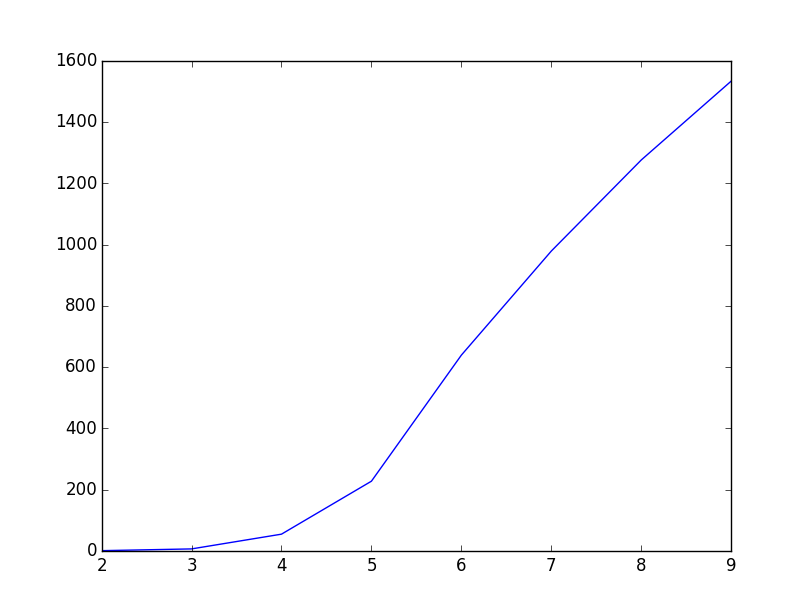
\includegraphics[scale=0.35]{explosion_dimensio_nb_calcul.png}
		\caption{algorithme 1 : Visualisation de l'explosion du temps de calcul en fonction de la dimension}
 	 	\end{center}  
		\vfill\hspace*{0mm}
	\end{figure}	
	
	
	\subsubsection{Isolation des points}
Afin de comprendre les origines du phénomène précédent, on a tracé l'évolution du nombre de cellules que contenait la table de hachage en fonction de la dimension et de la taille de chaque cellule.
  	\begin{figure}[h!]	
		\hspace*{0mm}\vfill
		\begin{center}	
		\includegraphics[scale=0.30]{figure_12.png}
		\caption{Evolution de la longueur de la table de hachage en fontion de epsilon et de la dimension (fléau de la dimension)}
  	 	\end{center}  
		\vfill\hspace*{0mm}	
	\end{figure}

\subsection{$3^{eme}$ expériences : évolution du coup}
Cette expérience avait pour objectif de traduire les valeurs prises par une certaine fonction de coût en fonction de l'évolution de l'algorithme.\\
Pour notre expérience, la fonction de coût est la suivante : $c(R = [p1, p2]) = distance(p1, p2)$. Dans notre cas, la distance en question dépend de la norme-2\\

	\begin{figure}[h!]
		\hspace*{0mm}\vfill
		\begin{center}		
		\includegraphics[scale=0.3]{exp_4_1000_10_2D.png}
		\caption{Evolution du coût en fonction de l'évolution de l'algorithme pour 1000 points et 10 clusters en 2 dimensions}
 	 	\end{center}  
		\vfill\hspace*{0mm}	
	\end{figure}
  	\begin{figure}[h!]
		\hspace*{0mm}\vfill
		\begin{center}
		\includegraphics[scale=0.3]{exo4_1000_10_3.png}	
		\caption{Evolution du coût en fonction de l'évolution de l'algorithme pour 1000 points et 10 cluters en 3 dimensions}
 		\end{center}  
		\vfill\hspace*{0mm}
	\end{figure}
  	\begin{figure}[h!]
		\hspace*{0mm}\vfill
		\begin{center}
		\includegraphics[scale=0.3]{exp_4_1000_10_4.png}	
		\caption{Evolution du coût en fonction de l'évolution de l'algorthme pour 1000 points et 10 cluters en 4  dimensions}
 		\end{center}  
		\vfill\hspace*{0mm}
	\end{figure}


\section{Evalutation des performances}
	Le deuxième algorithme de recherche des plus proches voisins est beaucoup plus rapide que l'ancien. On montre un tableau qui compare 
	leurs performances pour 1000 points puis on testera l'algorithme optimisé afin de voir ses limites.

	\begin{table}[!ht]
		\center
		\begin{tabular}{|c|c|c|}
	  	\hline
		Dimension & Temps algorithme Naïf (s) & Temps liste triée \\
	    \hline
		2 & 0.16 & 0.1\\
		3 & 11 & 4\\
		4 & 211 & 16\\
		5 & 2 151 & 81\\
		6 & 16 082 & 175 \\
		7 & ++ & 198 \\
		8 & ++ & 233\\
		\hline
		\end{tabular}	  
		\caption{Temps de calcul des deux algorithmes pour 1000 points et 10 clusters intiaux}
	\end{table}

	\begin{table}[!ht]
		\center
		\begin{tabular}{|c|c|}
	  	\hline
	  	Dimension & Temps (s) \\
	    \hline
		  2 & 0.49 \\
		  3 & 215\\
		  4 & 3 468\\
		  5 & 15 122 \\
		  6 & 33 017\\
		\hline
		\end{tabular}	  
		\caption{Algorithme optimisé : temps de calcul pour 5000 points et 50 clusters intiaux}
	\end{table}
  	\clearpage
 	\newpage
 	\mbox{~}
 	\clearpage
 	\newpage


	\part{conclusion}
						
	Pour conclure afin de résoudre le problème de clustering de données on a mis en place un algorithme composé de deux parties, une premiere parte permet de partitionner les points à l'ade d'une table de hachage, puis la seconde partie de l'algorithme fusionne petit à petit les clusters les plus proches afin d'en avoir un nombre optimal.
	Je remercie Thao et Nicolas pour leur aide et leur bienveillance tout au long de mon stage, je me remercie aussi l'equipe tempo et les equipes de VERIMAG pour leurs précieux conseils.
	  
	  \end{document}
